% ============================================================
% PhD PROGRESS REPORT PRESENTATION — NSUK CCS
% Isichei Nnamdi Augustus | PHD24DST0004
% ML-Enhanced Portfolio Optimisation for the NGX
% Template: copy of ../latex_proposal/Research_proposal.tex
% All figures are drawn from ../../results/ (see slide notes in comments)
% ============================================================
\documentclass[aspectratio=169,11pt]{beamer}
\PassOptionsToPackage{dvipsnames,svgnames,table}{xcolor}
\usepackage[utf8]{inputenc}
\usepackage[T1]{fontenc}
\usepackage{lmodern}
\usepackage{amsmath,amssymb,amsfonts}
\usepackage{graphicx}
\usepackage{booktabs}
\usepackage{natbib}
\usepackage{tikz}
\usepackage{pgfplots}
\pgfplotsset{compat=1.18}
\usetikzlibrary{shapes.geometric,arrows.meta,positioning,
	fit,backgrounds,calc,decorations.pathreplacing}
\usepackage{colortbl}
\usepackage{multirow}
\usepackage{bm}
\usepackage{qrcode}
\usepackage{array}
\newcolumntype{L}[1]{>{\raggedright\arraybackslash}p{#1}}

% ── COLOURS ────────────────────────────────────────────────
\definecolor{Navy}{HTML}{003366}
\definecolor{Gold}{HTML}{C49A00}
\definecolor{Green}{HTML}{006633}
\definecolor{Red}{HTML}{CC2200}
\definecolor{LightNavy}{HTML}{E8EEF5}
\definecolor{LightGold}{HTML}{FDF3D6}
\definecolor{LightGreen}{HTML}{E6F5ED}
\definecolor{LightRed}{HTML}{FDECEA}
\definecolor{SlateGray}{HTML}{607080}

% ── BEAMER THEME ───────────────────────────────────────────
\usetheme{Madrid}
\usecolortheme[named=Navy]{structure}
\setbeamercolor{palette primary}{bg=Navy,fg=white}
\setbeamercolor{palette secondary}{bg=Navy!85,fg=white}
\setbeamercolor{palette tertiary}{bg=Navy!70,fg=white}
\setbeamercolor{frametitle}{bg=Navy,fg=white}
\setbeamercolor{block title}{bg=Navy,fg=white}
\setbeamercolor{block body}{bg=LightNavy,fg=black}
\setbeamercolor{block title alerted}{bg=Red,fg=white}
\setbeamercolor{block body alerted}{bg=LightRed,fg=black}
\setbeamercolor{block title example}{bg=Green,fg=white}
\setbeamercolor{block body example}{bg=LightGreen,fg=black}
\setbeamercolor{itemize item}{fg=Gold}
\setbeamercolor{itemize subitem}{fg=Navy!70}
\setbeamerfont{frametitle}{size=\large,series=\bfseries}
\setbeamertemplate{navigation symbols}{}
\setbeamertemplate{itemize item}{\textbullet}
\setbeamertemplate{itemize subitem}{--}

% Gold underline on frametitle
\addtobeamertemplate{frametitle}{}{%
	\begin{tikzpicture}[remember picture,overlay]
		\draw[Gold,line width=2pt]
		(current page.north west) ++(0,-1.05cm) -- ++(16cm,0);
\end{tikzpicture}}

% Footer
\setbeamertemplate{footline}{
	\leavevmode\hbox{%
		\begin{beamercolorbox}[wd=.5\paperwidth,ht=2.25ex,dp=1ex,
			left,leftskip=1em]{palette primary}
			\tiny Isichei, N.A. | PHD24DST0004 | CCS-NSUK
		\end{beamercolorbox}%
		\begin{beamercolorbox}[wd=.3\paperwidth,ht=2.25ex,dp=1ex,
			center]{palette secondary}
			\tiny Progress Report -- ML Portfolio Optimisation, NGX
		\end{beamercolorbox}%
		\begin{beamercolorbox}[wd=.2\paperwidth,ht=2.25ex,dp=1ex,
			right,rightskip=1em]{palette primary}
			\tiny \insertframenumber{}/\inserttotalframenumber
\end{beamercolorbox}}}

% ── TIKZ STYLES (global — no #1 parameter) ─────────────────
\tikzset{
	arr/.style={-Stealth,thick,Navy},
	garr/.style={-Stealth,thick,Gold},
	navybox/.style={rectangle,draw=Navy,fill=LightNavy,
		rounded corners=3pt,inner sep=4pt,
		font=\scriptsize},
	greenbox/.style={rectangle,draw=Green,fill=LightGreen,
		rounded corners=3pt,inner sep=4pt,
		font=\scriptsize},
	redbox/.style={rectangle,draw=Red,fill=LightRed,
		rounded corners=3pt,inner sep=4pt,
		font=\scriptsize},
	goldbox/.style={rectangle,draw=Gold,fill=LightGold,
		rounded corners=3pt,inner sep=4pt,
		font=\scriptsize\bfseries},
}

% Shared chart style
\pgfplotsset{
	slide/.style={
		tick label style={font=\tiny},
		label style={font=\scriptsize},
		title style={font=\scriptsize\bfseries,color=Navy},
		legend style={font=\tiny,draw=none,fill=none},
		grid=major,grid style={gray!20},
		axis lines*=left,
	},
}

% ── CUSTOM COMMANDS ────────────────────────────────────────
\newcommand{\hl}[1]{\textcolor{Gold}{\textbf{#1}}}
\newcommand{\bE}{\mathbb{E}}
\newcommand{\bR}{\mathbb{R}}
\newcommand{\done}{\textcolor{Green}{\textbf{Done}}}
\newcommand{\proto}{\textcolor{Gold!80!black}{\textbf{Prototype}}}
\newcommand{\todo}{\textcolor{Red}{\textbf{Next}}}
% Status tag shown at the end of a frame title
\newcommand{\status}[1]{\hfill{\footnotesize\colorbox{Gold}{\textcolor{Navy}{\textbf{#1}}}}}
\newcommand{\appurl}{https://nairafolio-nine.vercel.app/}
% \textnaira (naira sign) is provided by textcomp under T1 encoding
% Logos are optional: the deck compiles without them
\newcommand{\logos}[1]{%
	\IfFileExists{nsuk_logo.jpg}{\includegraphics[height=#1]{nsuk_logo.jpg}\hspace{2cm}}{}%
	\IfFileExists{ccs_nsuk.jpg}{\includegraphics[height=#1]{ccs_nsuk.jpg}}{}}

% Abbreviation strip just above the footline (page-anchored; does not move slide content)
\newcommand{\abbr}[1]{%
	\begin{tikzpicture}[remember picture,overlay]
		\node[anchor=south west,inner sep=0pt,text width=15.2cm,align=left,
			font=\fontsize{5.6}{6.6}\selectfont,text=SlateGray]
			at ([xshift=0.4cm,yshift=0.42cm]current page.south west)
			{\textbf{\textcolor{Navy}{Abbreviations:}} #1};
	\end{tikzpicture}}

% ── META ───────────────────────────────────────────────────
\title[ML Portfolio Optimisation -- NGX]{%
	Machine Learning-Enhanced Portfolio Optimisation\\
	for Emerging Markets:\\
	A Two-Stage Approach for the Nigerian Stock Exchange}
\author[Isichei, N.A. | PHD24DST0004]{%
	\textbf{ISICHEI, Nnamdi Augustus} \\ {\small PHD24DST0004}}
\institute[CCS-NSUK]{%
	Centre for Cyberspace Studies\\
	Nasarawa State University, Keffi}
\date{PhD Progress Report, 2026}

% ===========================================================
\begin{document}
	% ===========================================================

	% ── SLIDE 1: TITLE ─────────────────────────────────────────
	{
		\setbeamertemplate{footline}{}
		\begin{frame}[plain]
			\begin{tikzpicture}[remember picture,overlay]
				\fill[Navy] (current page.south west) rectangle (current page.north east);
				\fill[Gold] (current page.north west) rectangle ++(16cm,-0.2cm);
				\fill[Navy!55] (current page.south west) rectangle ++(16cm,1.3cm);
			\end{tikzpicture}
			\vspace{0.15cm}
			\begin{center}
				\logos{1.4cm}\par\vspace{5pt}
				{\color{white}\rule{12cm}{0.4pt}}\\[8pt]
				{\color{Gold}\large\bfseries
					Machine Learning-Enhanced Portfolio Optimisation\\
					for Emerging Markets}\\[5pt]
				{\color{white}\normalsize
					A Two-Stage Approach for the Nigerian Stock Exchange}\\[10pt]
				{\color{white}\rule{8cm}{0.3pt}}\\[6pt]
				{\color{white}\small\bfseries ISICHEI, Nnamdi Augustus}\\
				{\color{white!75}\small PHD24DST0004 $\cdot$ Supervisor: Prof.\ H.\,K.\ Oduwole | Dr. \ S.\,E.\ Chaku}\\[4pt]
				{\color{white!65}\footnotesize
					Centre for Cyberspace Studies, Nasarawa State University, Keffi}\\[4pt]
				{\color{Gold!80}\footnotesize PhD Progress Report $\cdot$ 2026}
			\end{center}
		\end{frame}
	}

	% ── SLIDE 2: OUTLINE ───────────────────────────────────────
	\begin{frame}{Presentation Outline}
		\begin{columns}
			\column{0.48\textwidth}
			\tableofcontents[sections={1-4}]
			\column{0.48\textwidth}
			\tableofcontents[sections={5-7}]
		\end{columns}
	\end{frame}

	% ===========================================================
	\section{Problem Statement}
	% ===========================================================

	% ── SLIDE 3: PROBLEM STATEMENT ─────────────────────────────
	\begin{frame}{Problem Statement}
		\vspace{-14pt}
		\begin{alertblock}{Core Research Problem}
			\footnotesize Classical portfolio methods assume normal returns, stable volatility and liquid markets; the NGX violates all three.
			ML portfolio frameworks are validated on developed and Asian markets \citep{huang2024,orra2025}, not on African frontier exchanges \citep{adeabah2023african}.
		\end{alertblock}
		\vspace{-8pt}
		\begin{columns}[T]
			\column{0.49\textwidth}
			\begin{block}{Why classical methods struggle}
				\scriptsize
				\begin{itemize}\setlength\itemsep{1pt}
					\item \textbf{Fat tails:} 39/39 stocks non-normal (Jarque--Bera test)
					\item \textbf{Persistent volatility:} GARCH(1,1) persistence $\approx 0.90$
					\item \textbf{Thin, episodic trading:} volume comes in bursts
					\item \textbf{Oil and naira shocks:} regime-driven volatility
					\item \textbf{MVO estimation error} \citep{demiguel2009optimal}
				\end{itemize}
				\vspace{1pt}
				{\tiny First four: NGX findings of this research \citep{isichei2026characterising}}
			\end{block}
			\column{0.49\textwidth}
			\begin{exampleblock}{Gaps this study addresses}
				\scriptsize
				\begin{itemize}\setlength\itemsep{1pt}
					\item No validated \textbf{two-stage GNN--RL} framework for the NGX
					\item Stock-network structure unexploited \citep{patel2024}
					\item RL untested under NGX costs \citep{ngo2023frontier}
					\item Sentiment's \textbf{portfolio value} untested \citep{john2022}
					\item NGX never characterised for ML design
				\end{itemize}
			\end{exampleblock}
		\end{columns}
		\vspace{2pt}
		\begin{center}
			\colorbox{Navy}{\color{white}\footnotesize\bfseries\; Aim: design, validate and deploy an NGX-specific two-stage GAT--PPO portfolio framework \;}
		\end{center}
		\abbr{NGX: Nigerian Exchange; ML: Machine Learning; GARCH: Generalised Autoregressive Conditional Heteroskedasticity; MVO: Mean-Variance Optimisation; GNN: Graph Neural Network; RL: Reinforcement Learning; GAT: Graph Attention Network; PPO: Proximal Policy Optimisation.}
	\end{frame}

	% ===========================================================
	\section{Progress Since the Proposal}
	% ===========================================================

	% ── SLIDE 3: PROGRESS AT A GLANCE ──────────────────────────
	\begin{frame}{Progress at a Glance: Proposal Defense $\rightarrow$ Today}
		\vspace{-10pt}
		{\footnotesize\setlength{\tabcolsep}{4pt}\renewcommand{\arraystretch}{0.95}
		\begin{tabular}{L{2.6cm}L{3.9cm}L{5.5cm}c}
			\toprule
			\textbf{Research question} & \textbf{At proposal defense (Jun 2026)} & \textbf{Now (Oct 2026)} & \textbf{Status}\\
			\midrule
			\textbf{RQ4} NGX characterisation & 22 stocks, 2015--2025; paper under review & \textbf{Published}, PMLR Vol.\ 319; panel expanded to 39 stocks, 2012--2025 & \done\\[2pt]
			\textbf{RQ1} GAT pre-selection & Design only & GAT + 2 baselines, 7 walk-forward folds; best quintile spread (2.22\%/month) & \proto\\[2pt]
			\textbf{RQ2} RL allocation & Design only & PPO + MVO + equal weight, 68 out-of-sample months; Sharpe 1.077 & \proto\\[2pt]
			\textbf{RQ3} Sentiment & Conditional & 1,954 headlines scored; no significant gain ($t=-0.82$, $p\approx0.41$) & \done\\[2pt]
			\textbf{Artefact} & -- & \textbf{Nairafolio} robo-advisor deployed (GAT + PPO API) & \done\\
			\bottomrule
		\end{tabular}}
		\vspace{2pt}
		\begin{exampleblock}{In one sentence}
			\footnotesize The full pipeline (data $\rightarrow$ models $\rightarrow$ walk-forward evaluation $\rightarrow$ deployed advisor) now runs end to end; models are competitive with benchmarks but not yet clearly superior.
		\end{exampleblock}
		\abbr{RQ: Research Question; NGX: Nigerian Exchange; PMLR: Proceedings of Machine Learning Research; GAT: Graph Attention Network; RL: Reinforcement Learning; PPO: Proximal Policy Optimisation; MVO: Mean-Variance Optimisation; API: Application Programming Interface; $t$: t-statistic; $p$: p-value.}
	\end{frame}

	% ── SLIDE 4: WHAT CHANGED ──────────────────────────────────
	\begin{frame}{What Changed Since the Proposal, and Why}
		\vspace{-12pt}
		{\scriptsize\setlength{\tabcolsep}{4pt}\renewcommand{\arraystretch}{0.92}
		\begin{tabular}{L{1.9cm}L{3.9cm}L{4.9cm}L{3.0cm}}
			\toprule
			\textbf{Area} & \textbf{Proposed} & \textbf{Implemented} & \textbf{Reason}\\
			\midrule
			Sample & 2015--2025, 30--50 stocks & 2012--2025, 39 PIT NGX-30 stocks (incl.\ former) & Longer; no survivorship bias\\
			Validation & 5 rolling windows & 7 annual folds (2019--25), 68 test months & More out-of-sample data\\
			GAT & 3 layers, 8 heads, ranking loss & 2 layers, 2 heads, MSE on rank & Prototype; small data\\
			RQ1 baselines & LSTM, RF, XGBoost, TA & Random Forest, 60-day momentum & Prototype scope\\
			RL & DQN + multi-reward PPO & PPO; reward = return $-$ 10 bps & PPO suits continuous weights\\
			Two-stage link & GAT top-$K$ $\rightarrow$ RL & Tested separately; joined in advisor & Validate each stage first\\
			Macro data & Model inputs & Collected; used in RQ4 only & Price-based prototype\\
			Sentiment & BusinessDay, Nairametrics, Vanguard & Google News + GDELT (VADER) & No historical archives\\
			Metrics & Sharpe, Sortino, Calmar, CVaR, DM & Sharpe, CAGR, max DD, turnover, IC & Others planned\\
			\bottomrule
		\end{tabular}}
		\abbr{PIT: point-in-time; NGX-30: index of the 30 largest Nigerian Exchange stocks; GAT: Graph Attention Network; MSE: Mean Squared Error; LSTM: Long Short-Term Memory; RF: Random Forest; XGBoost: Extreme Gradient Boosting; TA: Technical Analysis; RL: Reinforcement Learning; DQN: Deep Q-Network; PPO: Proximal Policy Optimisation; bps: basis points (0.01\%); top-$K$: $K$ highest-ranked stocks; GDELT: Global Database of Events, Language and Tone; VADER: Valence Aware Dictionary and sEntiment Reasoner; CVaR: Conditional Value at Risk; DM: Diebold--Mariano; CAGR: Compound Annual Growth Rate; DD: Drawdown; IC: Information Coefficient.}
	\end{frame}

	% ===========================================================
	\section{Implemented Framework}
	% ===========================================================

	% ── SLIDE 5: PIPELINE ──────────────────────────────────────
	\begin{frame}{Implemented Pipeline and Validation}
		\begin{center}
		\vspace{-10pt}
		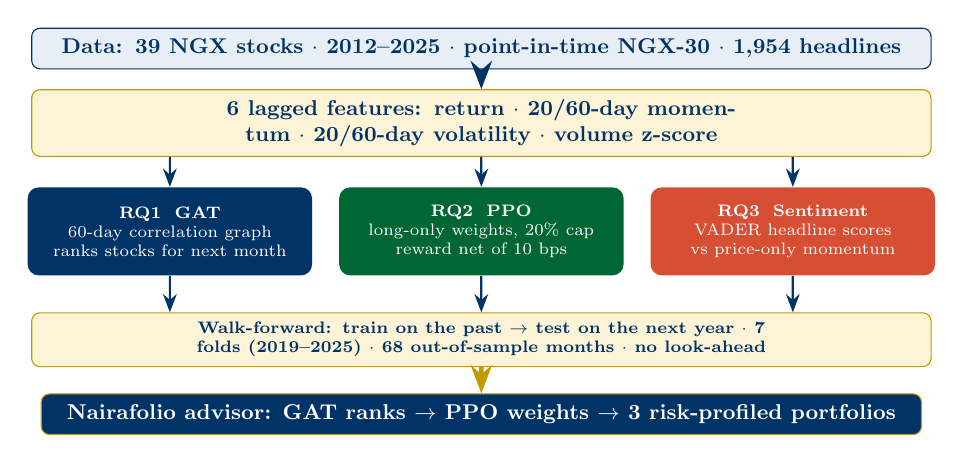
\begin{tikzpicture}[scale=0.86,transform shape]
			\node[navybox,text width=13cm,minimum height=0.6cm,align=center,font=\small\bfseries,text=Navy] (d) at (7,5.2)
			{Data: 39 NGX stocks $\cdot$ 2012--2025 $\cdot$ point-in-time NGX-30 $\cdot$ 1,954 headlines};
			\node[goldbox,text width=13cm,minimum height=0.55cm,align=center,font=\small\bfseries,text=Navy] (f) at (7,4.1)
			{6 lagged features: return $\cdot$ 20/60-day momentum $\cdot$ 20/60-day volatility $\cdot$ volume z-score};
			\draw[arr,ultra thick] (d) -- (f);

			\node[rectangle,fill=Navy,text=white,rounded corners=4pt,minimum width=4.2cm,minimum height=1.3cm,font=\scriptsize,align=center] (g) at (2.4,2.5)
			{\textbf{RQ1 \;GAT}\\60-day correlation graph\\ranks stocks for next month};
			\node[rectangle,fill=Green,text=white,rounded corners=4pt,minimum width=4.2cm,minimum height=1.3cm,font=\scriptsize,align=center] (p) at (7,2.5)
			{\textbf{RQ2 \;PPO}\\long-only weights, 20\% cap\\reward net of 10 bps};
			\node[rectangle,fill=Red!80,text=white,rounded corners=4pt,minimum width=4.2cm,minimum height=1.3cm,font=\scriptsize,align=center] (s) at (11.6,2.5)
			{\textbf{RQ3 \;Sentiment}\\VADER headline scores\\vs price-only momentum};
			\draw[arr] (f.south -| g) -- (g);
			\draw[arr] (f) -- (p);
			\draw[arr] (f.south -| s) -- (s);

			\node[goldbox,text width=13cm,minimum height=0.6cm,align=center,font=\scriptsize\bfseries,text=Navy] (w) at (7,0.9)
			{Walk-forward: train on the past $\rightarrow$ test on the next year $\cdot$ 7 folds (2019--2025) $\cdot$ 68 out-of-sample months $\cdot$ no look-ahead};
			\draw[arr] (g) -- (g |- w.north);
			\draw[arr] (p) -- (w);
			\draw[arr] (s) -- (s |- w.north);

			\node[rectangle,draw=Gold,fill=Navy,text=white,rounded corners=3pt,minimum width=13cm,minimum height=0.6cm,font=\small\bfseries] (a) at (7,-0.2)
			{Nairafolio advisor: GAT ranks $\rightarrow$ PPO weights $\rightarrow$ 3 risk-profiled portfolios};
			\draw[garr,ultra thick] (w) -- (a);
		\end{tikzpicture}
		\end{center}
		\vspace{-10pt}
		{\scriptsize\textcolor{SlateGray}{GAT and PPO are evaluated separately in the experiments; joining them inside the model is the next phase.}}
		\abbr{NGX-30: index of the 30 largest Nigerian Exchange stocks; RQ: Research Question; GAT: Graph Attention Network; PPO: Proximal Policy Optimisation; VADER: Valence Aware Dictionary and sEntiment Reasoner; bps: basis points (0.01\%).}
	\end{frame}

	% ===========================================================
	\section{Findings}
	% ===========================================================

	% ── SLIDE 6: RQ4 ───────────────────────────────────────────
	\begin{frame}{RQ4 -- The NGX Is Structurally Different \status{Published}}
		\vspace{-10pt}
		\begin{columns}[T]
			\column{0.47\textwidth}
			\begin{block}{Five findings (now $\cdot$ 39 stocks)}
				\footnotesize
				\begin{itemize}\setlength\itemsep{1pt}
					\item \textbf{Non-normal:} 39/39 fail Jarque--Bera; kurtosis 4.66
					\item \textbf{Persistent volatility:} GARCH $\alpha+\beta = 0.90$
					\item \textbf{Episodic liquidity:} 26\% above 75th-pctl CoV
					\item \textbf{Sparse links:} mean $\rho=0.07$; banks $\bar\rho=0.25$
					\item \textbf{High naira Sharpe}; naira $-$90\% vs USD
				\end{itemize}
				\vspace{1pt}
				{\tiny At proposal (22 stocks): kurtosis 4.79, GARCH 0.912, $\bar\rho=0.109$ \citep{isichei2026characterising}}
			\end{block}

			\column{0.5\textwidth}
			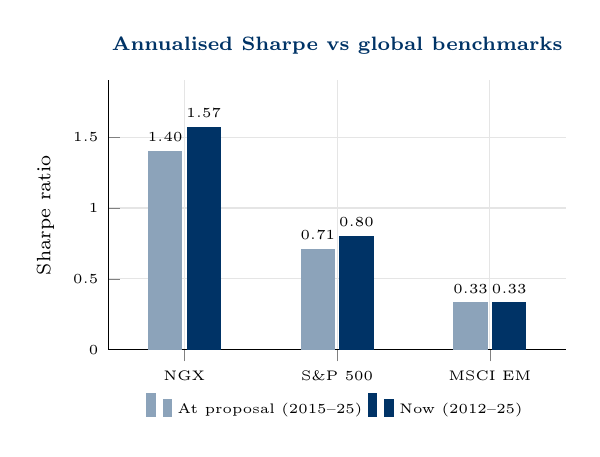
\begin{tikzpicture}
				\begin{axis}[slide,
					width=7.4cm,height=5.0cm,
					ybar,bar width=0.42cm,
					symbolic x coords={NGX,S\&P 500,MSCI EM},
					xtick=data,
					ymin=0,ymax=1.9,
					ylabel={Sharpe ratio},
					title={Annualised Sharpe vs global benchmarks},
					nodes near coords,
					nodes near coords style={font=\tiny,/pgf/number format/fixed,/pgf/number format/fixed zerofill,/pgf/number format/precision=2},
					legend style={at={(0.5,-0.14)},anchor=north,legend columns=2},
					enlarge x limits=0.25,
					]
					\addplot[fill=Navy!45,draw=Navy!45] coordinates {(NGX,1.40)(S\&P 500,0.71)(MSCI EM,0.33)};
					\addplot[fill=Navy,draw=Navy] coordinates {(NGX,1.57)(S\&P 500,0.80)(MSCI EM,0.33)};
					\legend{At proposal (2015--25),Now (2012--25)}
				\end{axis}
			\end{tikzpicture}
		\end{columns}
		\abbr{RQ: Research Question; NGX: Nigerian Exchange; GARCH: Generalised Autoregressive Conditional Heteroskedasticity ($\alpha+\beta$: volatility persistence); CoV: Coefficient of Variation; pctl: percentile; $\rho$: Pearson correlation; USD: US dollar; S\&P 500: Standard \& Poor's 500 index; MSCI EM: Morgan Stanley Capital International Emerging Markets index.}
	\end{frame}

	% ── SLIDE 7: RQ1 ───────────────────────────────────────────
	\begin{frame}{RQ1 -- GAT Pre-Selection vs Baselines \status{Prototype}}
		\vspace{-8pt}
		\begin{columns}[T]
			\column{0.33\textwidth}
			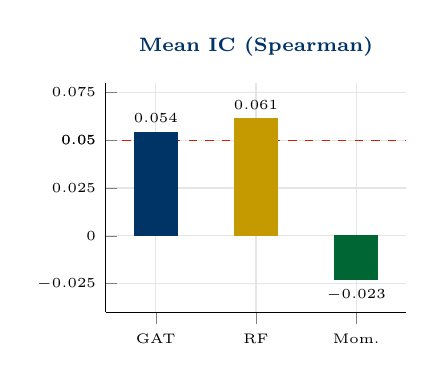
\begin{tikzpicture}
				\begin{axis}[slide,
					width=5.4cm,height=4.5cm,
					ybar,bar width=0.55cm,
					symbolic x coords={GAT,RF,Mom.},
					xtick={GAT,RF,Mom.},bar shift=0pt,scaled y ticks=false,
					ymin=-0.04,ymax=0.08,
					ytick={-0.025,0,0.025,0.05,0.075},
					yticklabel style={/pgf/number format/fixed,/pgf/number format/precision=3},
					title={Mean IC (Spearman)},
					nodes near coords,
					nodes near coords style={font=\tiny,/pgf/number format/fixed,/pgf/number format/precision=3},
					enlarge x limits=0.25,
					extra y ticks={0.05},extra y tick style={grid=major,major grid style={Red,dashed}},
					]
					\addplot[fill=Navy,draw=Navy] coordinates {(GAT,0.054)};
					\addplot[fill=Gold,draw=Gold] coordinates {(RF,0.061)};
					\addplot[fill=Green,draw=Green] coordinates {(Mom.,-0.023)};
				\end{axis}
			\end{tikzpicture}
			\column{0.33\textwidth}
			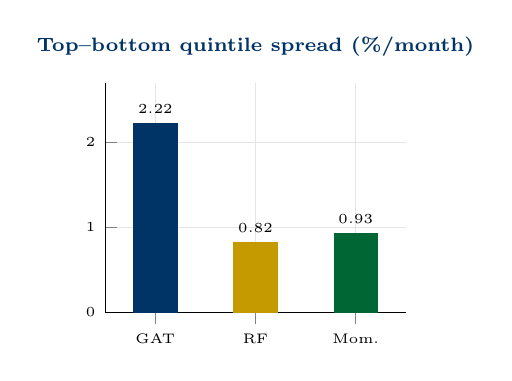
\begin{tikzpicture}
				\begin{axis}[slide,
					width=5.4cm,height=4.5cm,
					ybar,bar width=0.55cm,
					symbolic x coords={GAT,RF,Mom.},
					xtick={GAT,RF,Mom.},bar shift=0pt,scaled y ticks=false,
					ymin=0,ymax=2.7,
					title={Top--bottom quintile spread (\%/month)},
					nodes near coords,
					nodes near coords style={font=\tiny},
					enlarge x limits=0.25,
					]
					\addplot[fill=Navy,draw=Navy] coordinates {(GAT,2.22)};
					\addplot[fill=Gold,draw=Gold] coordinates {(RF,0.82)};
					\addplot[fill=Green,draw=Green] coordinates {(Mom.,0.93)};
				\end{axis}
			\end{tikzpicture}
			\column{0.32\textwidth}
			\begin{block}{Reading}
				\scriptsize
				\begin{itemize}\setlength\itemsep{2pt}
					\item GAT: \textbf{widest spread}: its top picks beat its bottom picks most
					\item RF: slightly \textbf{higher IC}, positive in 7/7 folds (GAT 6/7)
					\item Momentum \textbf{fails} on the NGX (IC $<0$)
					\item GAT median spread 1.54\%; 2022 lifts the mean
				\end{itemize}
			\end{block}
			\begin{alertblock}{Verdict}
				\scriptsize ML beats technical analysis; GAT vs RF not yet significant (1 seed).
			\end{alertblock}
		\end{columns}
		\vspace{-2pt}
		\parbox{0.64\textwidth}{\tiny\textcolor{SlateGray}{Means of 7 folds (2019--2025); dashed line: IC = 0.05. GAT \citep{velickovic2019}; RF \citep{breiman2001random}; Mom.\ \citep{jegadeesh1993returns}.}}
		\abbr{RQ: Research Question; GAT: Graph Attention Network; RF: Random Forest; Mom.: 60-day Momentum; IC: Information Coefficient; NGX: Nigerian Exchange; ML: Machine Learning; seed: random initialisation of a model run.}
	\end{frame}

	% ── SLIDE 8: RQ2 WEALTH ────────────────────────────────────
	\begin{frame}{RQ2 -- PPO Allocation vs MVO and Equal Weight \status{Prototype}}
		\vspace{-8pt}
		\begin{columns}[T]
			\column{0.58\textwidth}
			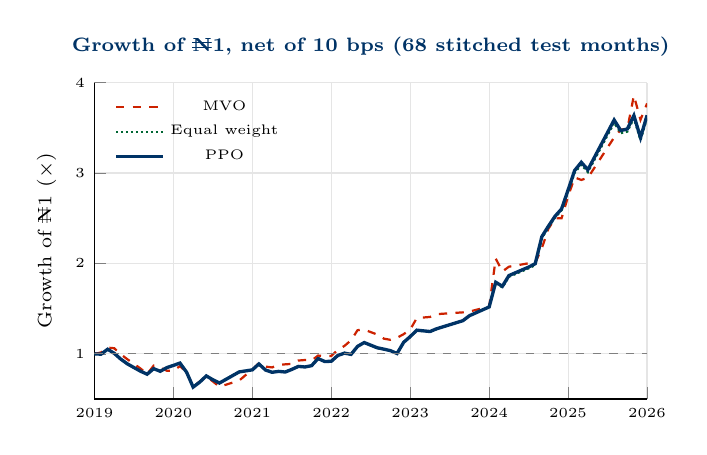
\begin{tikzpicture}
				\begin{axis}[slide,
					width=8.6cm,height=5.6cm,
					xmin=2019,xmax=2026,
					xtick={2019,...,2026},
					xticklabel style={/pgf/number format/1000 sep=},
					ymin=0.5,ymax=4,
					ylabel={Growth of \textnaira1 ($\times$)},
					title={Growth of \textnaira1, net of 10 bps (68 stitched test months)},
					legend style={at={(0.02,0.98)},anchor=north west},
					]
					\addplot[Red,thick,dashed] coordinates {(2019.0,1.000) (2019.083,1.015) (2019.167,1.069) (2019.250,1.062) (2019.333,0.996) (2019.417,0.940) (2019.583,0.838) (2019.667,0.776) (2019.750,0.870) (2019.833,0.850) (2019.917,0.813) (2020.000,0.815) (2020.083,0.864) (2020.167,0.797) (2020.250,0.637) (2020.333,0.694) (2020.417,0.748) (2020.500,0.695) (2020.583,0.636) (2020.833,0.705) (2021.000,0.827) (2021.083,0.898) (2021.167,0.859) (2021.250,0.850) (2021.333,0.877) (2021.417,0.884) (2021.500,0.889) (2021.583,0.926) (2021.667,0.932) (2021.750,0.926) (2021.833,0.981) (2021.917,0.974) (2022.000,0.977) (2022.083,1.045) (2022.167,1.088) (2022.250,1.150) (2022.333,1.262) (2022.417,1.268) (2022.583,1.213) (2022.667,1.168) (2022.750,1.155) (2022.833,1.178) (2022.917,1.218) (2023.000,1.269) (2023.083,1.396) (2023.250,1.408) (2023.333,1.439) (2023.667,1.459) (2023.750,1.468) (2024.000,1.523) (2024.083,2.054) (2024.167,1.911) (2024.250,1.964) (2024.500,2.002) (2024.583,2.007) (2024.667,2.169) (2024.750,2.383) (2024.833,2.498) (2024.917,2.500) (2025.000,2.743) (2025.083,2.951) (2025.167,2.924) (2025.250,2.947) (2025.583,3.394) (2025.667,3.481) (2025.750,3.489) (2025.833,3.857) (2025.917,3.589) (2026.000,3.770)};
					\addplot[Green,thick,densely dotted] coordinates {(2019.0,1.000) (2019.083,0.995) (2019.167,1.050) (2019.250,1.006) (2019.333,0.942) (2019.417,0.889) (2019.583,0.808) (2019.667,0.774) (2019.750,0.836) (2019.833,0.808) (2019.917,0.848) (2020.000,0.874) (2020.083,0.900) (2020.167,0.798) (2020.250,0.634) (2020.333,0.689) (2020.417,0.758) (2020.500,0.715) (2020.583,0.680) (2020.833,0.802) (2021.000,0.825) (2021.083,0.890) (2021.167,0.823) (2021.250,0.798) (2021.333,0.807) (2021.417,0.801) (2021.500,0.830) (2021.583,0.863) (2021.667,0.857) (2021.750,0.871) (2021.833,0.949) (2021.917,0.916) (2022.000,0.920) (2022.083,0.984) (2022.167,1.010) (2022.250,0.993) (2022.333,1.081) (2022.417,1.123) (2022.583,1.063) (2022.667,1.050) (2022.750,1.033) (2022.833,1.002) (2022.917,1.127) (2023.000,1.188) (2023.083,1.258) (2023.250,1.244) (2023.333,1.273) (2023.667,1.369) (2023.750,1.422) (2024.000,1.517) (2024.083,1.786) (2024.167,1.734) (2024.250,1.852) (2024.500,1.946) (2024.583,1.982) (2024.667,2.280) (2024.750,2.397) (2024.833,2.507) (2024.917,2.588) (2025.000,2.796) (2025.083,3.004) (2025.167,3.092) (2025.250,3.010) (2025.583,3.555) (2025.667,3.442) (2025.750,3.458) (2025.833,3.606) (2025.917,3.364) (2026.000,3.611)};
					\addplot[Navy,very thick] coordinates {(2019.0,1.000) (2019.083,0.996) (2019.167,1.051) (2019.250,1.006) (2019.333,0.942) (2019.417,0.889) (2019.583,0.808) (2019.667,0.775) (2019.750,0.836) (2019.833,0.807) (2019.917,0.848) (2020.000,0.872) (2020.083,0.898) (2020.167,0.797) (2020.250,0.632) (2020.333,0.687) (2020.417,0.756) (2020.500,0.713) (2020.583,0.677) (2020.833,0.800) (2021.000,0.823) (2021.083,0.888) (2021.167,0.821) (2021.250,0.796) (2021.333,0.806) (2021.417,0.799) (2021.500,0.828) (2021.583,0.861) (2021.667,0.855) (2021.750,0.869) (2021.833,0.948) (2021.917,0.915) (2022.000,0.918) (2022.083,0.982) (2022.167,1.008) (2022.250,0.994) (2022.333,1.083) (2022.417,1.125) (2022.583,1.067) (2022.667,1.052) (2022.750,1.035) (2022.833,1.004) (2022.917,1.128) (2023.000,1.191) (2023.083,1.262) (2023.250,1.247) (2023.333,1.277) (2023.667,1.367) (2023.750,1.422) (2024.000,1.519) (2024.083,1.792) (2024.167,1.747) (2024.250,1.866) (2024.500,1.960) (2024.583,1.997) (2024.667,2.296) (2024.750,2.412) (2024.833,2.521) (2024.917,2.603) (2025.000,2.814) (2025.083,3.029) (2025.167,3.119) (2025.250,3.036) (2025.583,3.587) (2025.667,3.470) (2025.750,3.487) (2025.833,3.636) (2025.917,3.392) (2026.000,3.639)};
					\addplot[gray,dashed,thin,forget plot] coordinates {(2019,1) (2026,1)};
					\legend{MVO,Equal weight,PPO}
				\end{axis}
			\end{tikzpicture}
			\column{0.4\textwidth}
			{\scriptsize
			\begin{tabular}{lrrr}
				\toprule
				& \textbf{PPO} & \textbf{MVO} & \textbf{EW}\\
				\midrule
				CAGR & 25.6\% & \textbf{26.4\%} & 25.4\%\\
				Sharpe & \textbf{1.077} & 1.024 & 1.072\\
				Max DD & $-$39.8\% & $-$40.5\% & $\mathbf{-39.6\%}$\\
				Turnover/mo & 15.2\% & 39.8\% & \textbf{13.4\%}\\
				\bottomrule
			\end{tabular}}
			\vspace{6pt}
			\begin{alertblock}{Key finding}
				\scriptsize PPO's monthly returns correlate \textbf{0.9999} with equal weight: the agent has \textbf{learned $1/N$}, a notoriously hard benchmark \citep{demiguel2009optimal}.
			\end{alertblock}
			{\tiny\textcolor{SlateGray}{Likely causes: 2,048 training steps per fold, return-only reward, no GAT input.}}
		\end{columns}
		\abbr{RQ: Research Question; PPO: Proximal Policy Optimisation; MVO: Mean-Variance Optimisation; EW: Equal Weight; CAGR: Compound Annual Growth Rate; Max DD: Maximum Drawdown; mo: month; bps: basis points (0.01\%); $1/N$: equal weighting across $N$ stocks; GAT: Graph Attention Network; \textnaira: naira.}
	\end{frame}

	% ── SLIDE 9: RQ2 COSTS ─────────────────────────────────────
	\begin{frame}{RQ2 -- Where PPO Already Wins: Cost Robustness}
		\vspace{-8pt}
		\begin{columns}[T]
			\column{0.58\textwidth}
			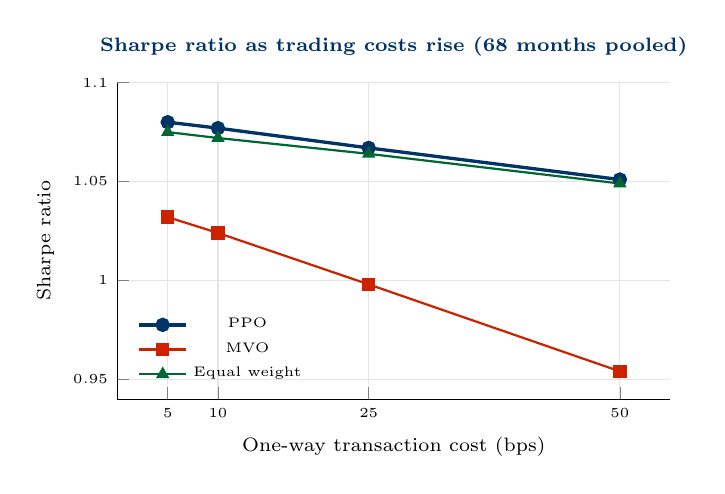
\begin{tikzpicture}
				\begin{axis}[slide,
					width=8.6cm,height=5.6cm,
					xmin=0,xmax=55,
					xtick={5,10,25,50},
					ymin=0.94,ymax=1.10,
					yticklabel style={/pgf/number format/fixed,/pgf/number format/precision=2},
					xlabel={One-way transaction cost (bps)},
					ylabel={Sharpe ratio},
					title={Sharpe ratio as trading costs rise (68 months pooled)},
					legend style={at={(0.02,0.02)},anchor=south west},
					]
					\addplot[Navy,very thick,mark=*] coordinates {(5,1.080)(10,1.077)(25,1.067)(50,1.051)};
					\addplot[Red,thick,mark=square*] coordinates {(5,1.032)(10,1.024)(25,0.998)(50,0.954)};
					\addplot[Green,thick,mark=triangle*] coordinates {(5,1.075)(10,1.072)(25,1.064)(50,1.049)};
					\legend{PPO,MVO,Equal weight}
				\end{axis}
			\end{tikzpicture}
			\column{0.4\textwidth}
			\begin{block}{Reading}
				\small
				\begin{itemize}\setlength\itemsep{3pt}
					\item 5 $\rightarrow$ 50 bps: PPO loses \textbf{0.029} Sharpe; MVO loses \textbf{0.078}
					\item At 50 bps PPO's CAGR (24.7\%) overtakes MVO's (24.1\%)
					\item Cause: PPO trades \textbf{2.6$\times$ less} than MVO
				\end{itemize}
			\end{block}
			\begin{exampleblock}{Implication for NGX investors}
				\small Real NGX dealing costs exceed 10 bps; low-turnover allocation keeps more of the return.
			\end{exampleblock}
		\end{columns}
		\abbr{RQ: Research Question; PPO: Proximal Policy Optimisation; MVO: Mean-Variance Optimisation; bps: basis points (0.01\%); CAGR: Compound Annual Growth Rate; NGX: Nigerian Exchange.}
	\end{frame}

	% ── SLIDE 10: RQ3 ──────────────────────────────────────────
	\begin{frame}{RQ3 -- Does News Sentiment Add Value? \status{Complete}}
		\vspace{-8pt}
		\begin{columns}[T]
			\column{0.36\textwidth}
			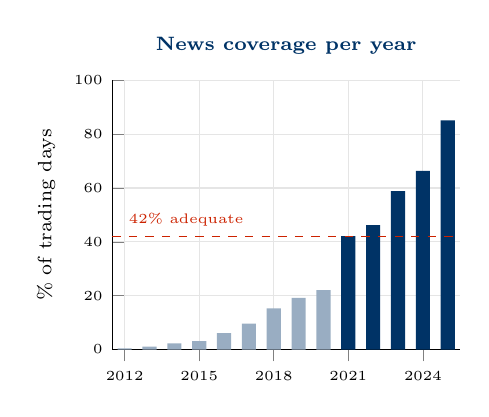
\begin{tikzpicture}
				\begin{axis}[slide,
					width=6.0cm,height=5.0cm,
					ybar,bar width=0.18cm,bar shift=0pt,
					xmin=2011.5,xmax=2025.5,
					xtick={2012,2015,2018,2021,2024},
					xticklabel style={/pgf/number format/1000 sep=},
					ymin=0,ymax=100,
					ylabel={\% of trading days},
					title={News coverage per year},
					]
					\addplot[fill=Navy!40,draw=none] coordinates {(2012,0.4)(2013,1.1)(2014,2.3)(2015,3.1)(2016,6.1)(2017,9.6)(2018,15.3)(2019,19.2)(2020,22.1)};
					\addplot[fill=Navy,draw=none] coordinates {(2021,42.1)(2022,46.2)(2023,58.8)(2024,66.4)(2025,85.1)};
					\draw[Red,dashed,thin] (axis cs:2011.5,42) -- (axis cs:2025.5,42) node[pos=0.02,above right,font=\tiny,Red] {42\% adequate};
				\end{axis}
			\end{tikzpicture}
			\column{0.32\textwidth}
			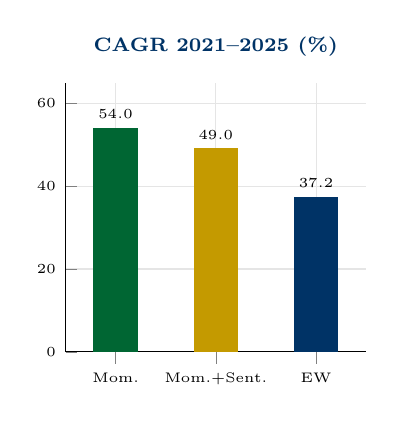
\begin{tikzpicture}
				\begin{axis}[slide,
					width=5.4cm,height=5.0cm,
					ybar,bar width=0.55cm,
					symbolic x coords={Mom.,Mom.+Sent.,EW},
					xtick={Mom.,Mom.+Sent.,EW},bar shift=0pt,
					ymin=0,ymax=65,
					title={CAGR 2021--2025 (\%)},
					nodes near coords,
					nodes near coords style={font=\tiny,/pgf/number format/fixed,/pgf/number format/fixed zerofill,/pgf/number format/precision=1},
					enlarge x limits=0.25,
					]
					\addplot[fill=Green,draw=Green] coordinates {(Mom.,54.0)};
					\addplot[fill=Gold,draw=Gold] coordinates {(Mom.+Sent.,49.0)};
					\addplot[fill=Navy,draw=Navy] coordinates {(EW,37.2)};
				\end{axis}
			\end{tikzpicture}
			\column{0.3\textwidth}
			\begin{block}{Result}
				\scriptsize
				\begin{itemize}\setlength\itemsep{2pt}
					\item Adding sentiment: \textbf{$-$3.45 pp/yr}
					\item 95\% CI $[-11.7\%, +4.8\%]$; HAC $t=-0.82$, $p\approx0.41$ \citep{newey1987simple}
					\item Full 2012--25 run agrees ($t=-0.42$); VADER scoring \citep{hutto2014vader}
					\item Equal weight: best Sharpe (1.639)
				\end{itemize}
			\end{block}
			\begin{alertblock}{Caveat}
				\scriptsize Sparse news before 2021; VADER is a general-purpose lexicon.
			\end{alertblock}
		\end{columns}
		\abbr{RQ: Research Question; Mom.: price-only Momentum; Sent.: Sentiment; EW: Equal Weight; CAGR: Compound Annual Growth Rate; pp: percentage points; CI: Confidence Interval; HAC: Heteroskedasticity and Autocorrelation Consistent; VADER: Valence Aware Dictionary and sEntiment Reasoner.}
	\end{frame}

	% ── SLIDE 11: SCOREBOARD ───────────────────────────────────
	\begin{frame}{Which Model Performs Best?}
		\vspace{-4pt}
		{\small
		\begin{tabular}{L{3.4cm}L{3.2cm}L{2.8cm}L{4.2cm}}
			\toprule
			\textbf{Contest} & \textbf{Winner} & \textbf{Runner-up} & \textbf{Verdict}\\
			\midrule
			Ranking accuracy (IC) & Random Forest 0.061 & GAT 0.054 & Close; RF more consistent\\
			Winners vs losers (spread) & \cellcolor{LightNavy}\textbf{GAT 2.22\%} & Momentum 0.93\% & GAT best where profit is made\\
			Risk-adjusted return & \cellcolor{LightNavy}\textbf{PPO 1.077} & Equal wt 1.072 & Practically a tie\\
			Raw return (CAGR) & MVO 26.4\% & PPO 25.6\% & MVO, at 2.6$\times$ the trading\\
			Cost robustness & \cellcolor{LightNavy}\textbf{PPO} & Equal weight & PPO degrades least\\
			Sentiment increment & Price-only & + Sentiment & No significant value\\
			\bottomrule
		\end{tabular}}
		\vspace{8pt}
		\begin{block}{Overall}
			\small Proposed models are \textbf{competitive but not yet clearly superior}: GAT shows the strongest promise; PPO currently reproduces equal weighting.
		\end{block}
		\abbr{IC: Information Coefficient; RF: Random Forest; GAT: Graph Attention Network; PPO: Proximal Policy Optimisation; MVO: Mean-Variance Optimisation; CAGR: Compound Annual Growth Rate; wt: weight.}
	\end{frame}

	% ===========================================================
	\section{Research Artefact \& Live Demo}
	% ===========================================================

	% ── SLIDE 12: NAIRAFOLIO ───────────────────────────────────
	\begin{frame}{From Research to Product: the Nairafolio Robo-Advisor}
		\vspace{-6pt}
		\begin{center}
		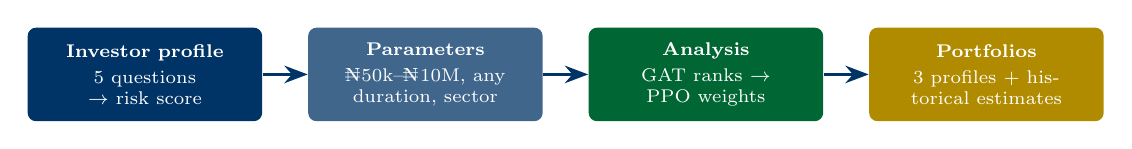
\begin{tikzpicture}[scale=0.95,transform shape]
			\foreach \i/\t/\s/\c in {
				0/Investor profile/5 questions $\rightarrow$ risk score/Navy,
				1/Parameters/{\textnaira50k--\textnaira10M, any duration, sector}/Navy!75,
				2/Analysis/GAT ranks $\rightarrow$ PPO weights/Green,
				3/Portfolios/{3 profiles + historical estimates}/Gold!90!black}{
				\node[rectangle,fill=\c,text=white,rounded corners=3pt,text width=2.9cm,minimum height=1.25cm,font=\scriptsize,align=center]
				(s\i) at (\i*3.75,0) {\textbf{\t}\\[2pt]\s};
			}
			\foreach \i/\j in {0/1,1/2,2/3}{\draw[arr,very thick] (s\i) -- (s\j);}
		\end{tikzpicture}
		\end{center}
		\vspace{2pt}
		\begin{columns}[T]
			\column{0.55\textwidth}
			{\scriptsize
			\begin{tabular}{lrrrr}
				\toprule
				\textbf{Profile} & \textbf{Stocks} & \textbf{CAGR} & \textbf{Sharpe} & \textbf{Worst fall}\\
				\midrule
				Conservative & 10 & 28.9\% & 1.12 & $-$30.2\%\\
				Moderate & 8 & 34.7\% & 1.10 & $-$37.5\%\\
				Aggressive & 5 & 35.4\% & 0.89 & $-$38.2\%\\
				\textcolor{SlateGray}{Full PPO} & \textcolor{SlateGray}{$\sim$30} & \textcolor{SlateGray}{25.6\%} & \textcolor{SlateGray}{1.08} & \textcolor{SlateGray}{$-$39.8\%}\\
				\bottomrule
			\end{tabular}}\\[2pt]
			{\tiny\textcolor{SlateGray}{Walk-forward replay of the saved models, 2019--2025, monthly rebalancing, 10 bps. Rule selected on the same months: estimates likely optimistic.}}
			\column{0.42\textwidth}
			\begin{block}{Built on the findings}
				\scriptsize
				\begin{itemize}\setlength\itemsep{1pt}
					\item Liquidity filter from \textbf{RQ4}
					\item Risk set by concentration: fewer stocks = more risk
					\item Monthly rebalancing, as validated
					\item Next.js app + FastAPI model service
				\end{itemize}
			\end{block}
		\end{columns}
		\abbr{GAT: Graph Attention Network; PPO: Proximal Policy Optimisation; CAGR: Compound Annual Growth Rate; RQ: Research Question; bps: basis points (0.01\%); \textnaira: naira; k: thousand; M: million; Next.js: web-app framework; FastAPI: Python web-service framework.}
	\end{frame}

	% ── SLIDE 13: LIVE DEMO ────────────────────────────────────
	{
		\setbeamertemplate{footline}{}
		\begin{frame}[plain]
			\begin{tikzpicture}[remember picture,overlay]
				\fill[Navy] (current page.south west) rectangle (current page.north east);
				\fill[Gold] (current page.north west) rectangle ++(16cm,-0.2cm);
			\end{tikzpicture}
			\begin{columns}[c]
				\column{0.58\textwidth}
				{\color{Gold}\Large\bfseries Live Demo}\\[6pt]
				{\color{white}\large Nairafolio: NGX Robo-Advisor}\\[14pt]
				{\color{white}\normalsize\href{\appurl}{\texttt{nairafolio-nine.vercel.app}}}\\[14pt]
				{\color{white!80}\small
				\begin{tabular}{@{}l@{\;\;}l}
					\textcolor{Gold}{1.} & Overview: headline results\\
					\textcolor{Gold}{2.} & Research: interactive figures\\
					\textcolor{Gold}{3.} & Advisor: \textnaira750,000 $\cdot$ 8 months $\cdot$ Oil \& Gas\\
				\end{tabular}}
				\column{0.36\textwidth}
				\begin{center}
					\colorbox{white}{\qrcode[height=3.6cm]{\appurl}}\\[6pt]
					{\color{white!70}\scriptsize Scan to try it yourself}
				\end{center}
			\end{columns}
		\end{frame}
	}

	% ===========================================================
	\section{Next Steps}
	% ===========================================================

	% ── SLIDE 14: GAP CHECK & ROADMAP ──────────────────────────
	\begin{frame}{Next Phase: Closing the Gaps and Sharpening Novelty}
		\vspace{-14pt}
		\begin{columns}[T]
			\column{0.5\textwidth}
			\begin{block}{RQ4 design requirements vs prototype}
				{\scriptsize\renewcommand{\arraystretch}{0.95}
				\begin{tabular}{@{}L{4.6cm}l@{}}
					Downside (drawdown/CVaR) reward & \textcolor{Red}{\textbf{Not yet}}\\
					GARCH / volatility-regime features & \textcolor{Gold!80!black}{\textbf{Partial}}\\
					Monthly rebalancing, NGX costs & \textcolor{Gold!80!black}{\textbf{Partial}}\\
					Attention checked on bank cluster & \textcolor{Gold!80!black}{\textbf{Partial}}\\
					Outlier exclusion (TRANSCORP) & \textcolor{Red}{\textbf{Not yet}}\\
				\end{tabular}}
			\end{block}
			\begin{exampleblock}{Target novelty}
				\scriptsize Liquidity- and macro-aware GAT informing a downside-risk PPO, validated walk-forward on a survivorship-free NGX panel.
			\end{exampleblock}
			\column{0.47\textwidth}
			\begin{block}{Prioritised improvements}
				\scriptsize
				\begin{enumerate}\setlength\itemsep{1pt}
					\item \textbf{Join the stages:} GAT scores in PPO's state \citep{huang2024}
					\item \textbf{Fix PPO:} 50k+ steps, downside reward, 5--10 seeds
					\item \textbf{NGX graph:} sector + liquidity + oil/FX context node; ranking loss
					\item \textbf{GAT + RF stack} to combine strengths
					\item \textbf{Statistics:} DM \citep{diebold1995comparing}, Sharpe test \citep{ledoit2008robust}; Sortino, Calmar, CVaR
					\item \textbf{Data:} total returns; USD and real-terms results
					\item \textbf{RQ3+:} FinBERT; sentiment as a GAT node feature
				\end{enumerate}
			\end{block}
		\end{columns}
		\abbr{RQ: Research Question; CVaR: Conditional Value at Risk; GARCH: Generalised Autoregressive Conditional Heteroskedasticity; NGX: Nigerian Exchange; TRANSCORP: Transnational Corporation Plc; GAT: Graph Attention Network; PPO: Proximal Policy Optimisation; RF: Random Forest; FX: foreign exchange; DM: Diebold--Mariano test; USD: US dollar; FinBERT: Financial Bidirectional Encoder Representations from Transformers; k: thousand.}
	\end{frame}

	% ── SLIDE 15: TIMELINE ─────────────────────────────────────
	\begin{frame}{Revised Timeline}
		\vspace{-2pt}
		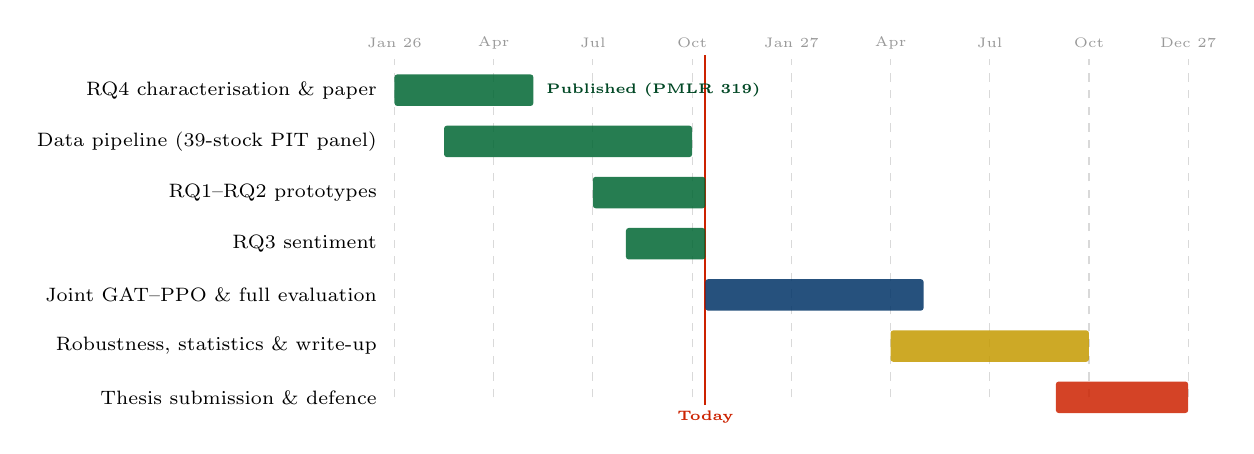
\begin{tikzpicture}
			% axis: Jan 2026 (0) to Dec 2027 (24); 0.42 cm per month, origin x=3.6
			\foreach \m/\lbl in {0/Jan 26,3/Apr,6/Jul,9/Oct,12/Jan 27,15/Apr,18/Jul,21/Oct,24/Dec 27}{
				\pgfmathsetmacro{\xg}{3.6 + \m*0.42}
				\draw[gray!30,dashed] (\xg,0.6) -- (\xg,4.9);
				\node[font=\tiny,gray!80] at (\xg,5.1) {\lbl};
			}
			% today marker (Oct 2026 = month 9.4)
			\pgfmathsetmacro{\xt}{3.6 + 9.4*0.42}
			\draw[Red,thick] (\xt,0.5) -- (\xt,4.95);
			\node[font=\tiny\bfseries,Red,fill=white,inner sep=1pt] at (\xt,0.35) {Today};

			\foreach \y/\lbl/\s/\e/\c/\p in {
				4.5/{RQ4 characterisation \& paper}/0/4.2/Green/Done,
				3.85/{Data pipeline (39-stock PIT panel)}/1.5/9/Green/Done,
				3.2/{RQ1--RQ2 prototypes}/6/9.4/Green/Done,
				2.55/{RQ3 sentiment}/7/9.4/Green/Done,
				1.9/{Joint GAT--PPO \& full evaluation}/9.4/16/Navy/Next,
				1.25/{Robustness, statistics \& write-up}/15/21/Gold/Next,
				0.6/{Thesis submission \& defence}/20/24/Red/Next}{
				\node[font=\scriptsize,anchor=east] at (3.5,\y) {\lbl};
				\pgfmathsetmacro{\xs}{3.6 + \s*0.42}
				\pgfmathsetmacro{\xe}{3.6 + \e*0.42}
				\fill[\c,opacity=0.85,rounded corners=1pt] (\xs,\y-0.2) rectangle (\xe,\y+0.2);
			}
			\node[font=\tiny\bfseries,Green!70!black,anchor=west] at (3.6+4.3*0.42,4.5) {Published (PMLR 319)};
		\end{tikzpicture}
		{\tiny\textcolor{SlateGray}{Green: completed $\cdot$ Navy/Gold/Red: remaining phases. Original plan: 24 months from January 2026.}}
		\abbr{RQ: Research Question; PIT: point-in-time; GAT: Graph Attention Network; PPO: Proximal Policy Optimisation; PMLR: Proceedings of Machine Learning Research.}
	\end{frame}

	% ===========================================================
	\section{References}
	% ===========================================================

	\begin{frame}[allowframebreaks]{Key References}
		\nocite{huang2024,velickovic2019,schulman2019,markowitz2024,orra2025,omorokunwa2023,lu2025,kipf2023,sutton2019,kumbure2022,espiga2024,liang2024portfolio,naeem2024ml,bekaert2007liquidity,bekaert2023globalized,emenike2021westafrica,
			aawaar2023african,ngene2022volume,adigwe2015stockmarket,wu2021comprehensive,
			kumeka2022stockafrica,jarque1987test,bollerslev1986generalized}
		\setbeamertemplate{bibliography item}[text]
		\bibliographystyle{apalike}
		{\tiny\bibliography{references_presentation}}
	\end{frame}

	% ── THANK YOU ───────────────────────────────────────────────
	{
		\setbeamertemplate{footline}{}
		\begin{frame}[plain]
			\begin{tikzpicture}[remember picture,overlay]
				\fill[Navy] (current page.south west) rectangle (current page.north east);
				\fill[Gold] (current page.north west) rectangle ++(16cm,-0.2cm);
				\fill[Navy!55] (current page.south west) rectangle ++(16cm,1.4cm);
			\end{tikzpicture}
			\begin{center}
				\vspace{0.5cm}
				\logos{1.3cm}\par\vspace{8pt}
				{\color{white}\rule{10cm}{0.4pt}}\\[10pt]
				{\color{Gold}\LARGE\bfseries Thank You}\\[8pt]
				{\color{white}\large Questions \& Discussion}\\[10pt]
				{\color{white}\rule{8cm}{0.3pt}}\\[6pt]
				{\color{white!85}\small\textbf{Isichei, Nnamdi Augustus}
					$\;\mid\;$ PHD24DST0004}\\[4pt]
				{\color{white!70}\footnotesize isicheinnamdi.com $\;\cdot\;$ nairafolio-nine.vercel.app}\\[4pt]
				{\color{white!70}\footnotesize Centre for Cyberspace Studies,
					Nasarawa State University, Keffi}\\[5pt]
				{\color{Gold!85}\footnotesize ``Knowledge for Development''}
			\end{center}
		\end{frame}
	}

\end{document}
